% (The MIT License)
%
% Copyright (c) 2023-2024 Yegor Bugayenko
%
% Permission is hereby granted, free of charge, to any person obtaining a copy
% of this software and associated documentation files (the 'Software'), to deal
% in the Software without restriction, including without limitation the rights
% to use, copy, modify, merge, publish, distribute, sublicense, and/or sell
% copies of the Software, and to permit persons to whom the Software is
% furnished to do so, subject to the following conditions:
%
% The above copyright notice and this permission notice shall be included in all
% copies or substantial portions of the Software.
%
% THE SOFTWARE IS PROVIDED 'AS IS', WITHOUT WARRANTY OF ANY KIND, EXPRESS OR
% IMPLIED, INCLUDING BUT NOT LIMITED TO THE WARRANTIES OF MERCHANTABILITY,
% FITNESS FOR A PARTICULAR PURPOSE AND NONINFRINGEMENT. IN NO EVENT SHALL THE
% AUTHORS OR COPYRIGHT HOLDERS BE LIABLE FOR ANY CLAIM, DAMAGES OR OTHER
% LIABILITY, WHETHER IN AN ACTION OF CONTRACT, TORT OR OTHERWISE, ARISING FROM,
% OUT OF OR IN CONNECTION WITH THE SOFTWARE OR THE USE OR OTHER DEALINGS IN THE
% SOFTWARE.

\documentclass{article}
\usepackage{../sqm}
\newcommand*\thetitle{Code Coverage}
\begin{document}

\plush{\sqmTitlePage{15}}

% Statement
% Branch/Decision
% Modified Condition/Decision Coverage (MC/DC)
% LCSAJ (Linear Code Sequence and Jump)


\pptBanner{Example, Part I}
\begin{multicols}{2}
Live Code:\par
{\small\begin{ffcode*}{highlightlines={1,5-6}}
int fibonacci(int n) {
  if (n <= 0) {
    return 0;
  }
  if (n <= 2) {
    return 1;
  }
  return fibonacci(n-1)
    + fibonacci(n-2);
}
\end{ffcode*}
}
\par\columnbreak\par
Test Code:\par
{\small\begin{ffcode*}{}
assert fibonacci(1) == 1;
assert fibonacci(2) == 1;
\end{ffcode*}
}
\( C = 3/10 = 30\% \)
\end{multicols}
\plush{}

\pptBanner{Example, Part I}
\begin{multicols}{2}
Live Code:\par
{\small\begin{ffcode*}{highlightlines={1,5-6,8-9}}
int fibonacci(int n) {
  if (n <= 0) {
    return 0;
  }
  if (n <= 2) {
    return 1;
  }
  return fibonacci(n-1)
    + fibonacci(n-2);
}
\end{ffcode*}
}
\par\columnbreak\par
Test Code:\par
{\small\begin{ffcode*}{}
assert fibonacci(1) == 1;
assert fibonacci(2) == 1;

assert fibonacci(9) == 34;
assert fibonacci(10) == 55;
\end{ffcode*}
}
\( C = 5/10 = 50\% \)
\end{multicols}
\plush{}

\pitch{\pptQuote{brian-marick.jpg}{Coverage numbers (like many numbers) are dangerous because they're \emph{objective} but \emph{incomplete}. They too often distort sensible action. Using them in isolation is as foolish as hiring based only on GPA.}{Brian Marick, \href{http://www.exampler.com/testing-com/writings/coverage.pdf}{\textit{How to Misuse Code Coverage}}, 1997}}

\pitch{\pptQuote{../06-coupling/martin-fowler.jpg}{I would be suspicious of anything like 100\% --- it would smell of someone writing tests to make the coverage \emph{numbers happy}, but not thinking about what they are doing.}{Martin Fowler, \href{https://martinfowler.com/bliki/TestCoverage.html}{\textit{Test Coverage}}, 1997}}

\pitch{\pptBanner{Codecov.io}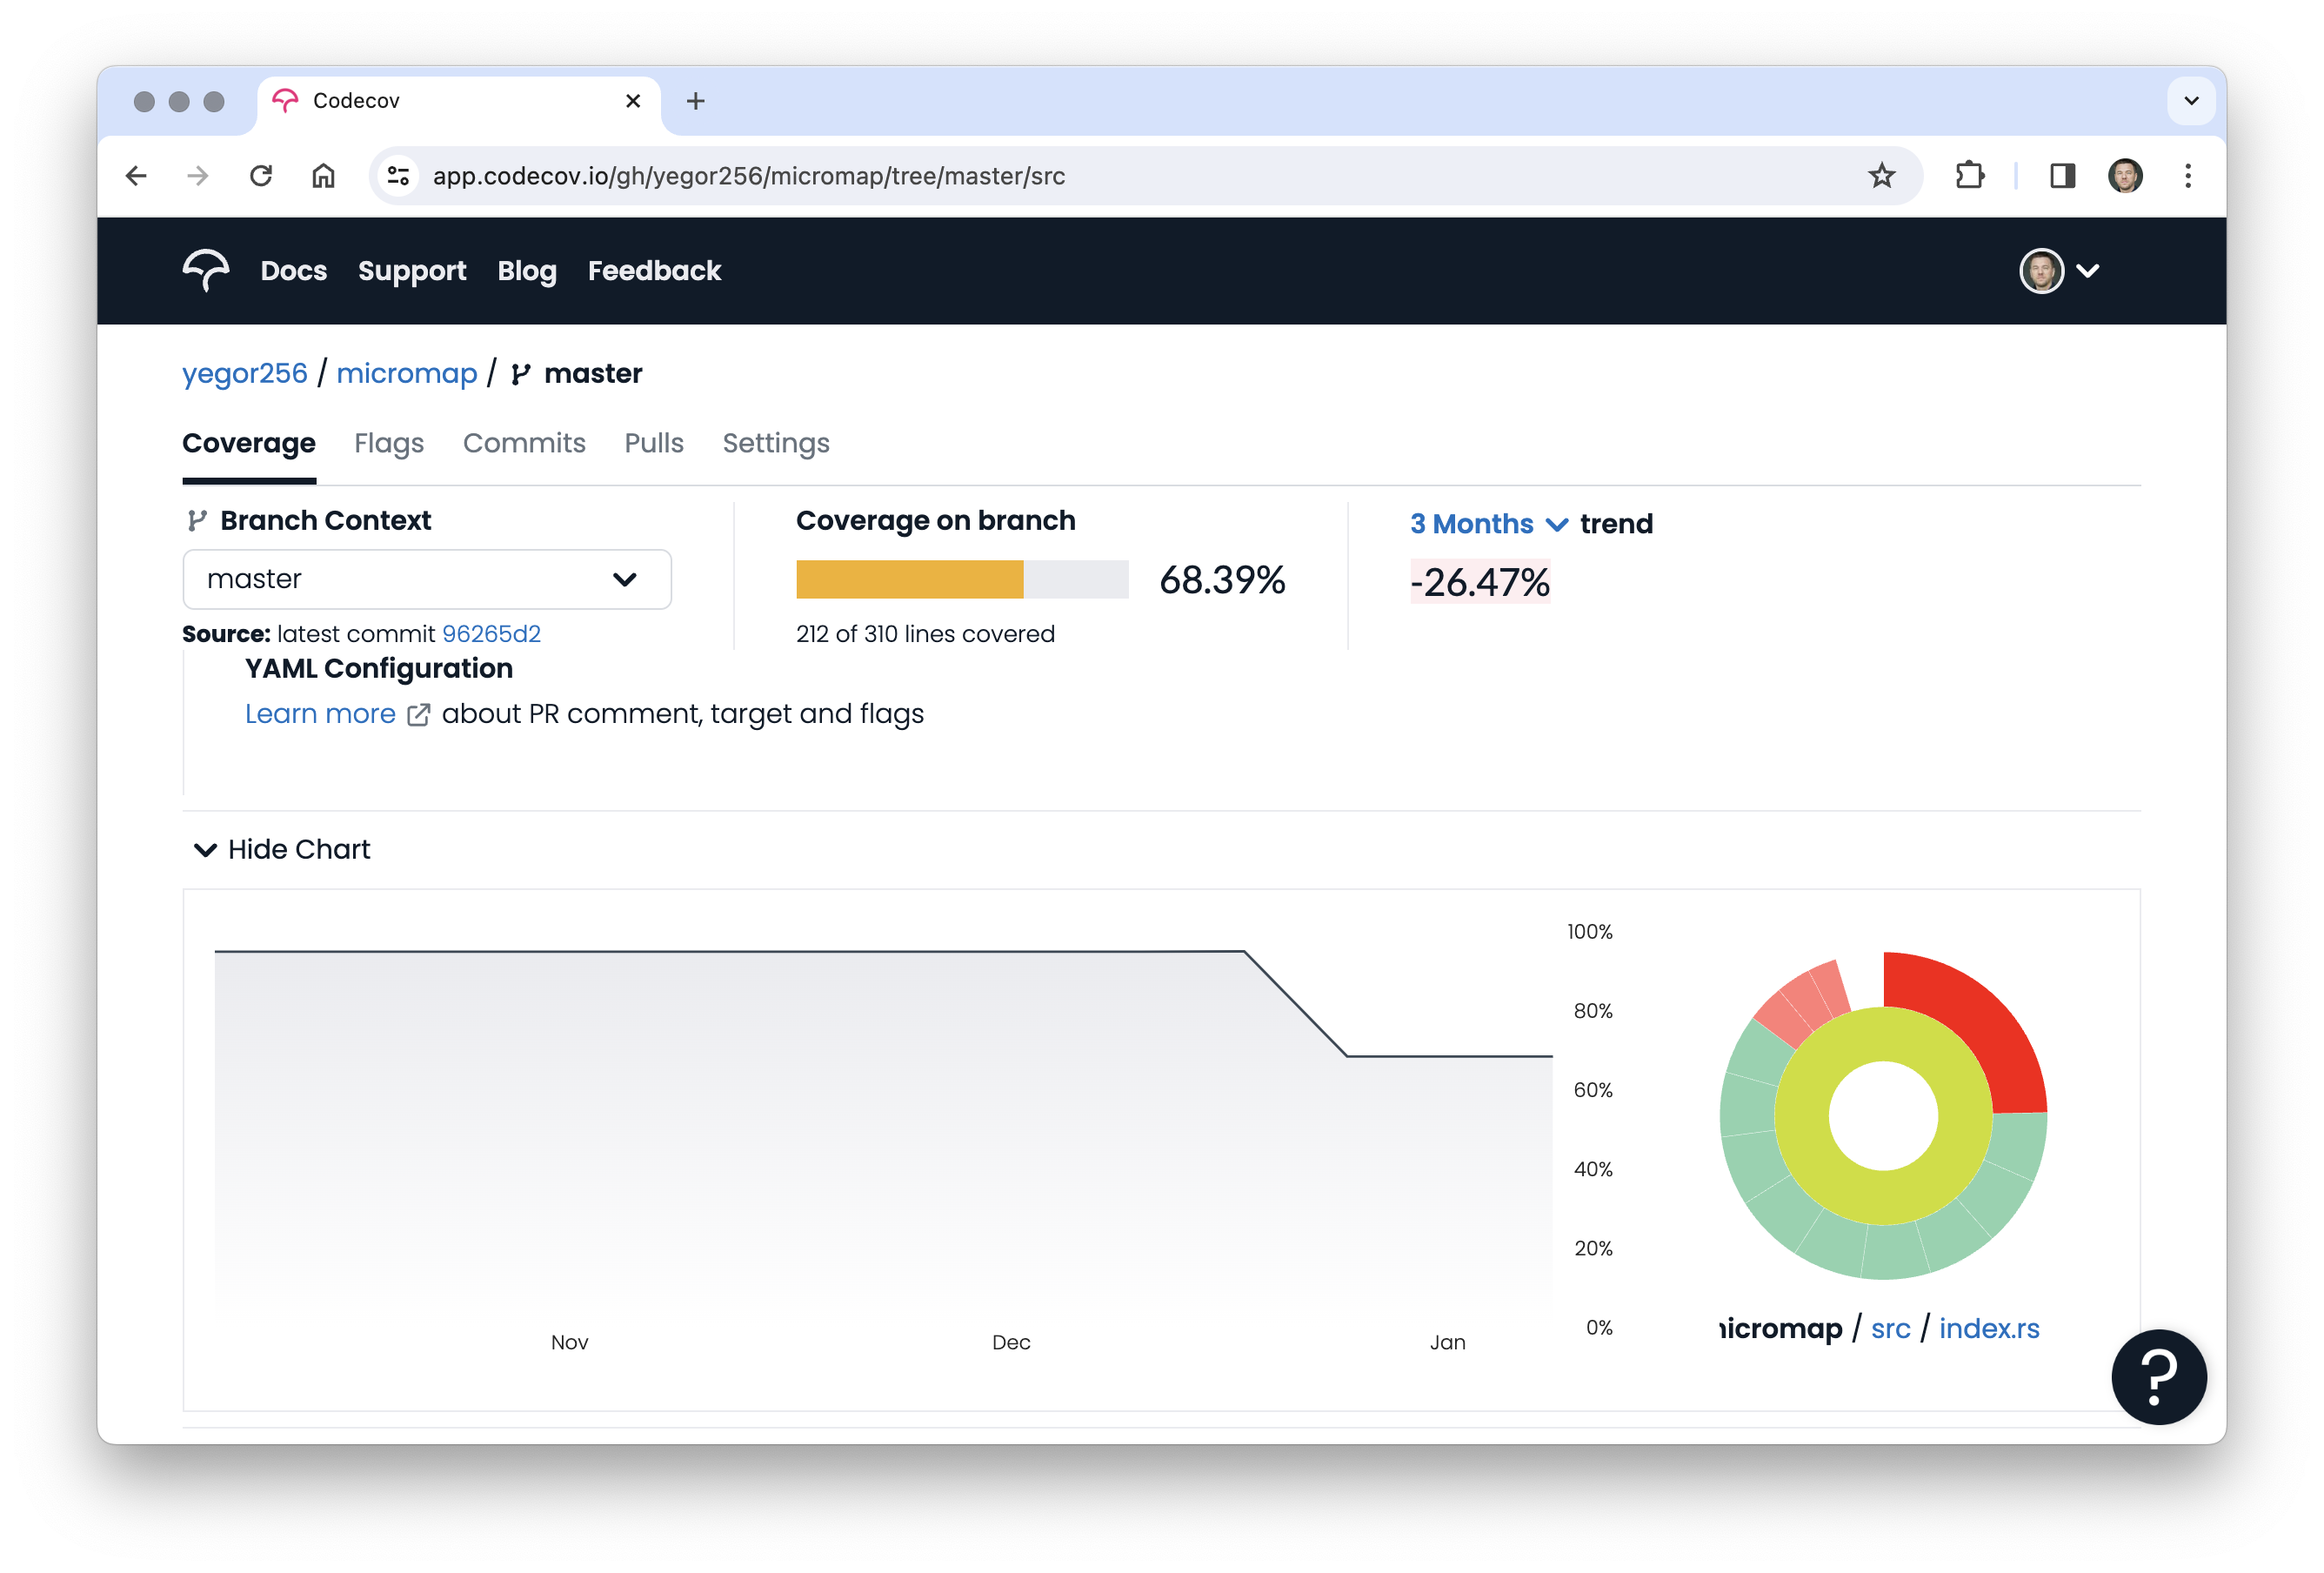
\includegraphics[width=.7\textwidth]{codecov.png}}

\pitch{\pptBanner{Line Coverage}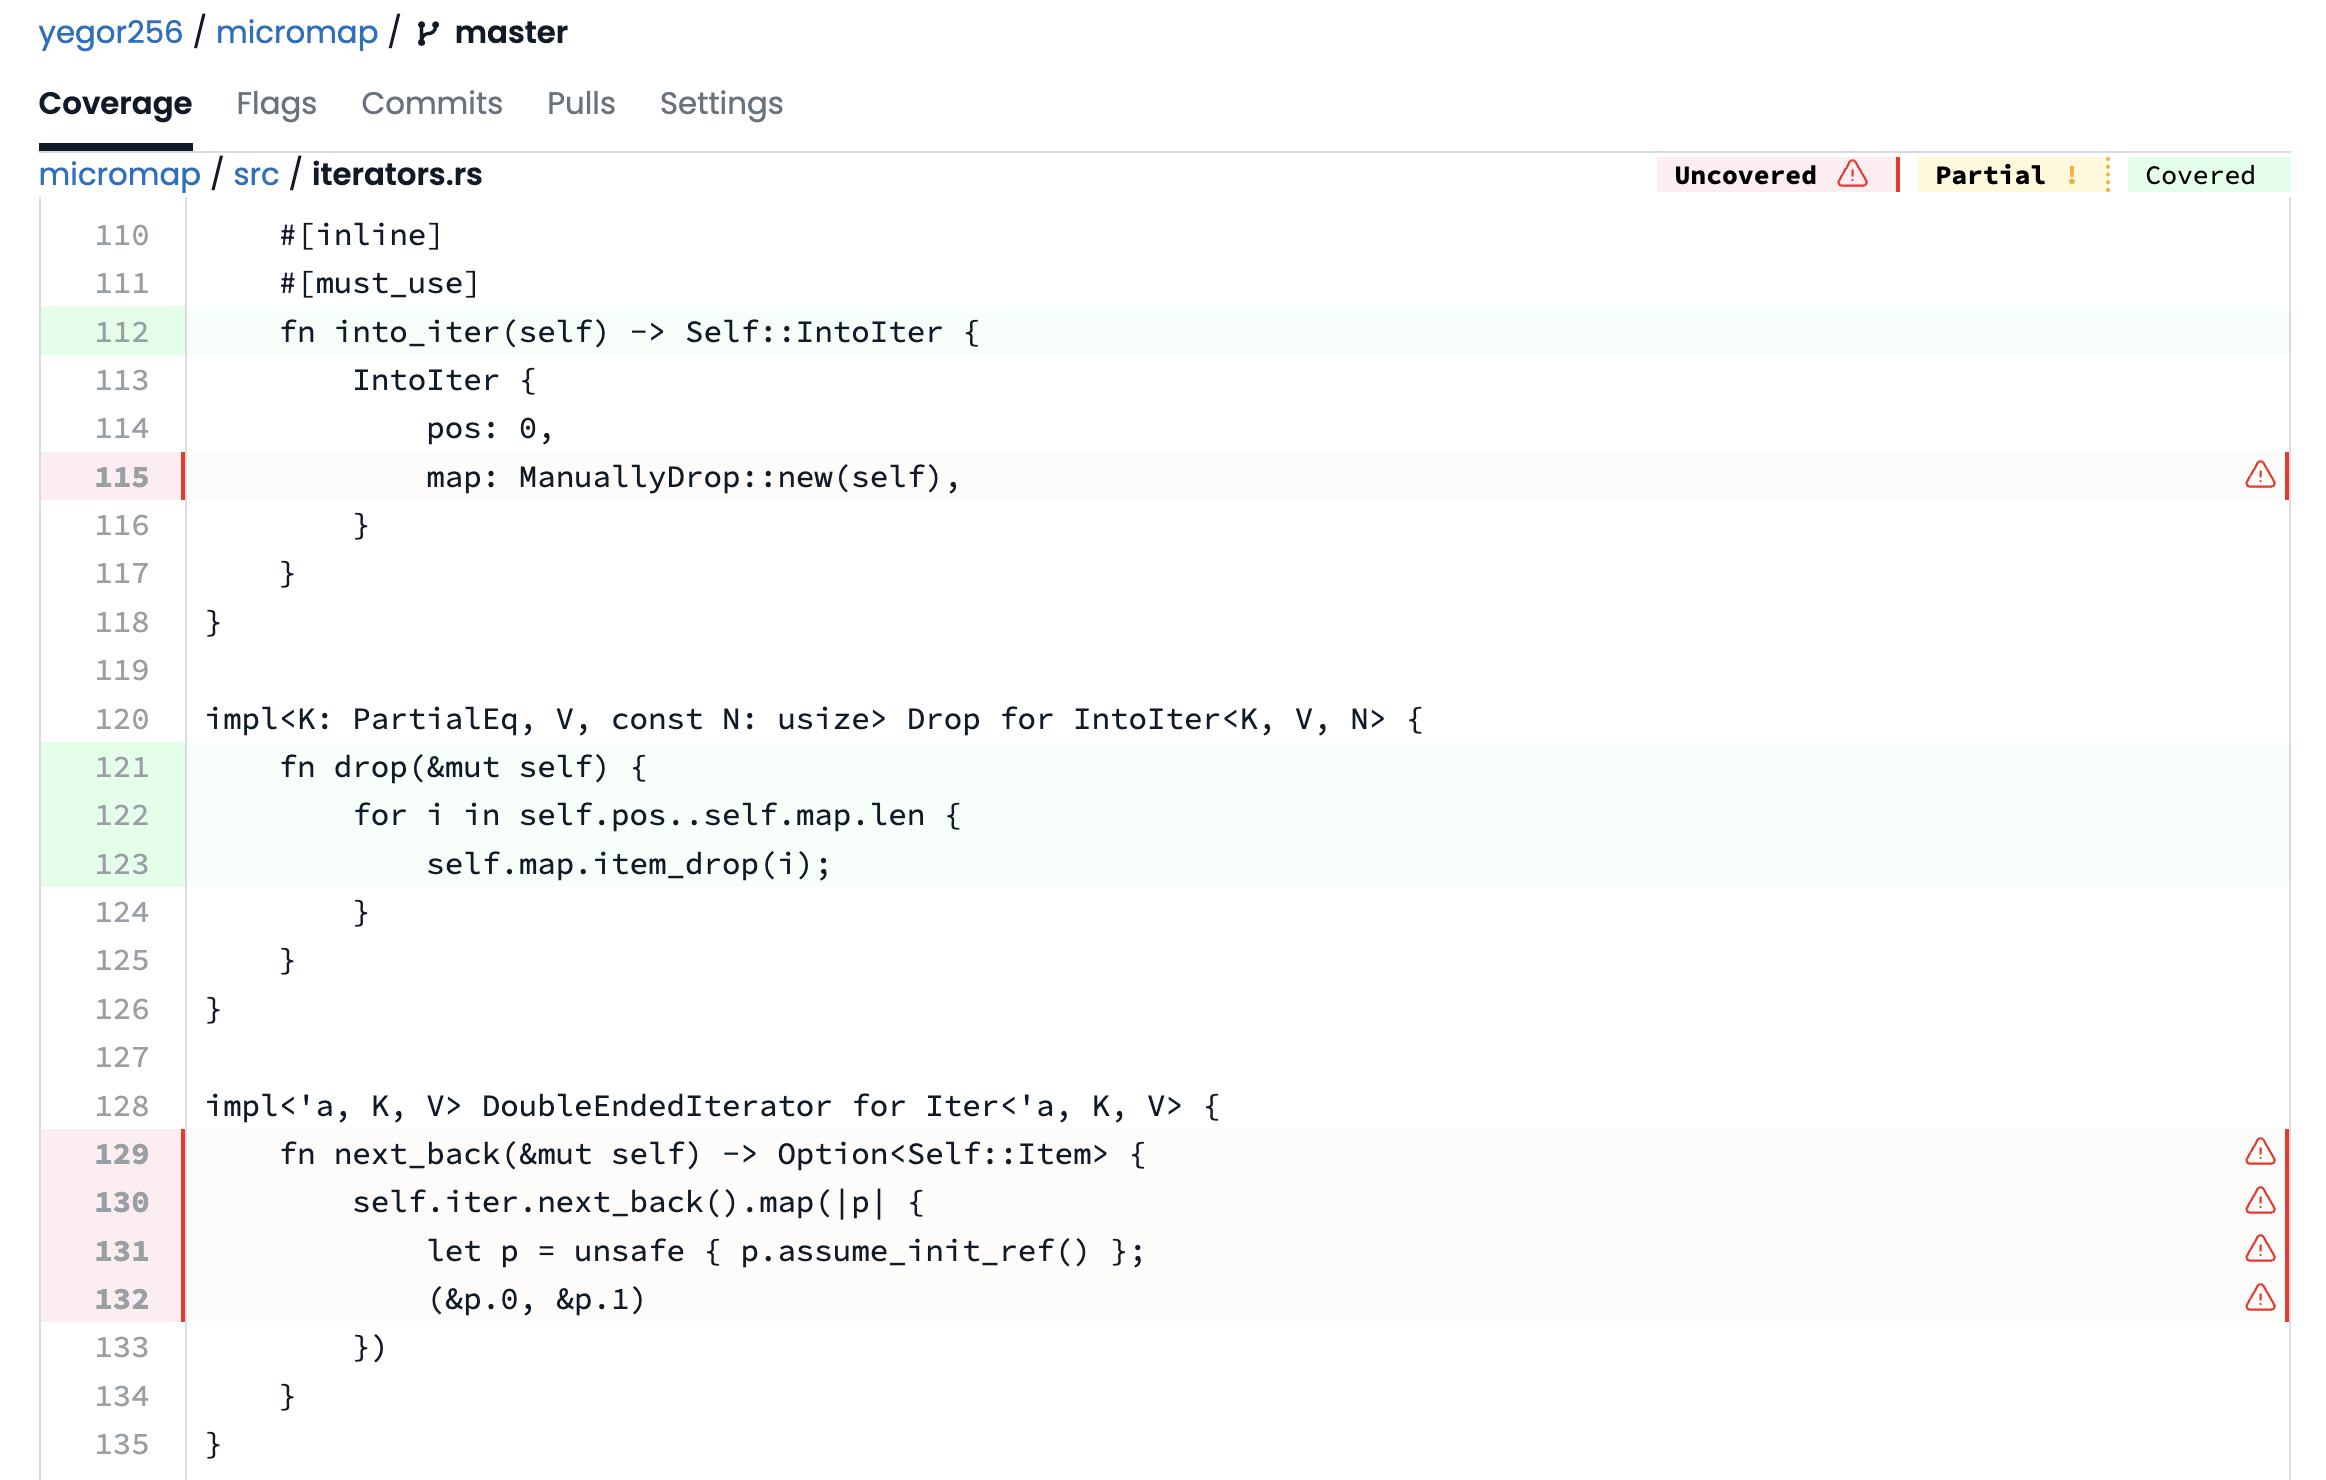
\includegraphics[width=.7\textwidth]{lines.png}}

\pitch{\pptBanner{Tarpaulin for Rust}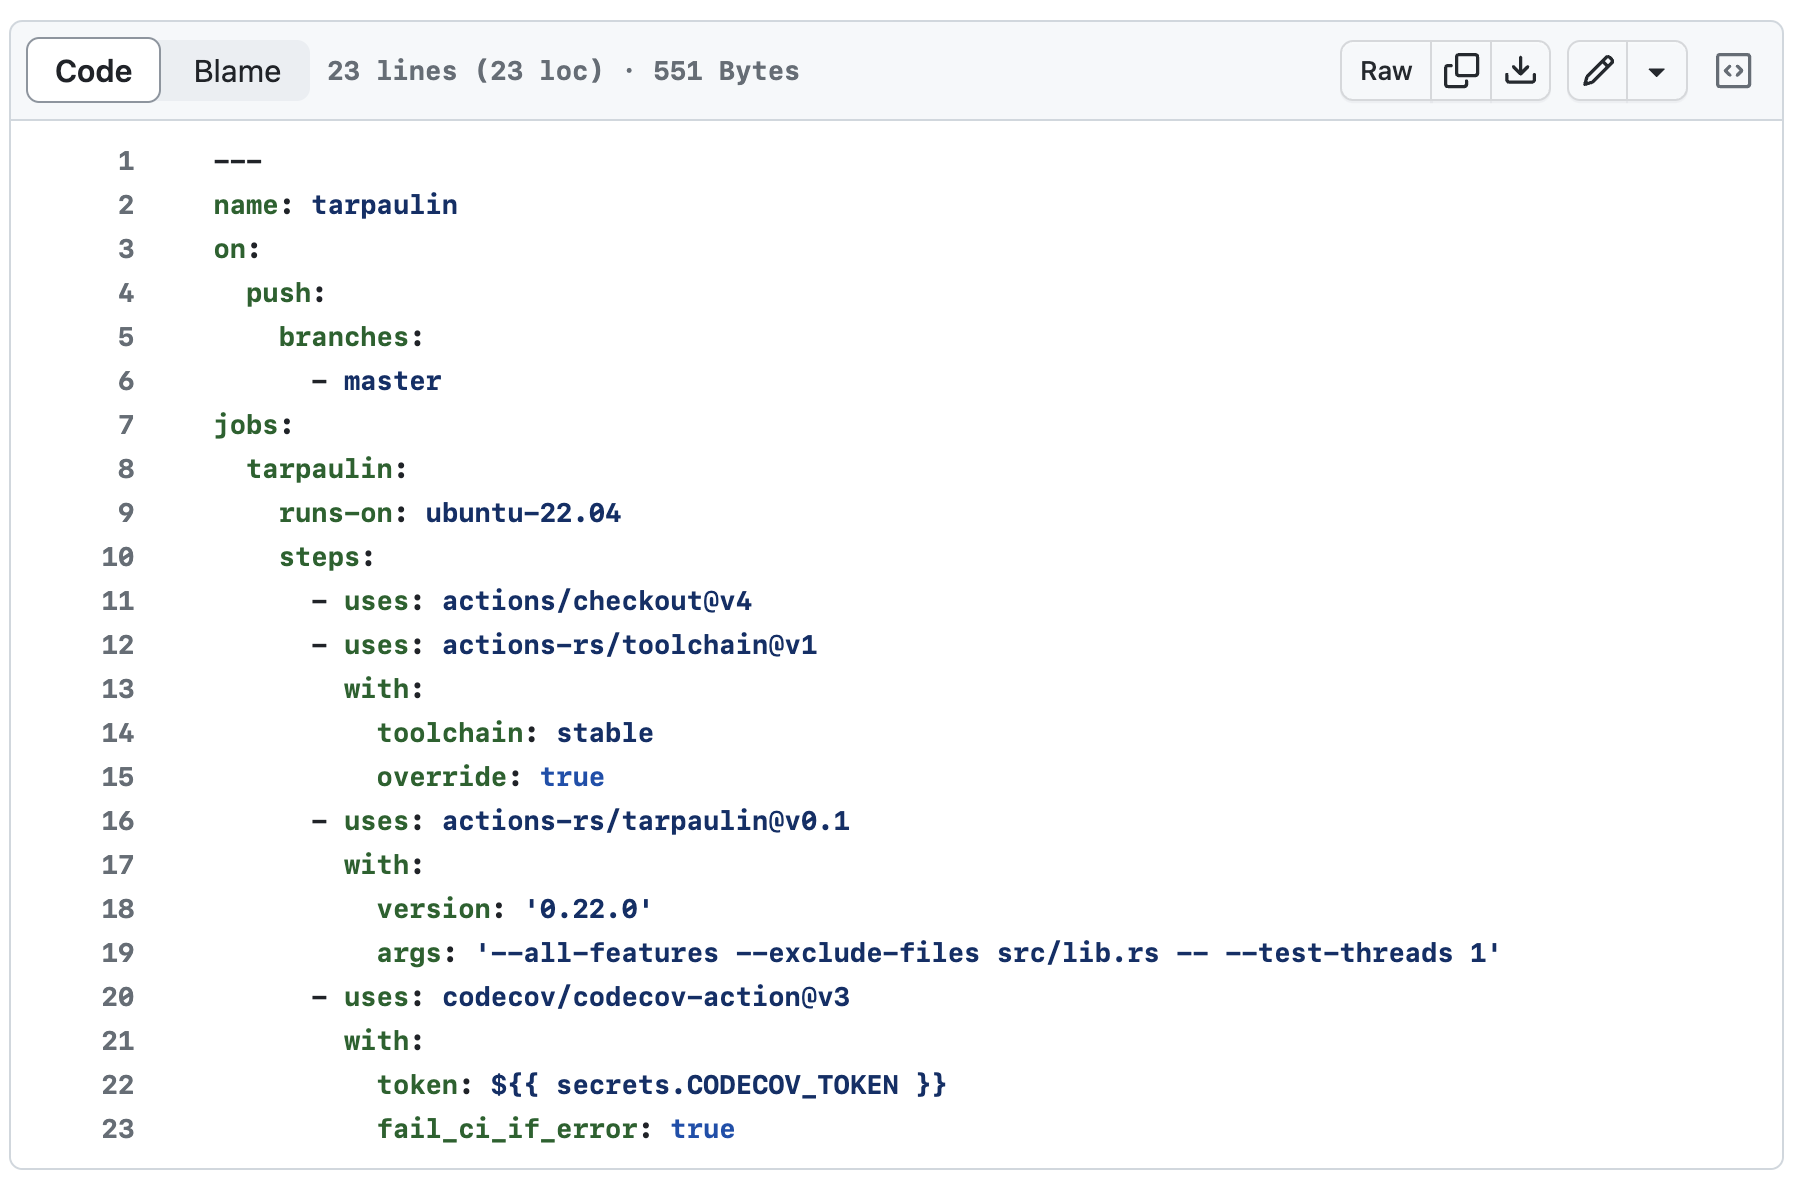
\includegraphics[width=.7\textwidth]{tarpaulin.png}}

\pitch{Code Coverage can be calculated by a few tools:
\begin{itemize}
\item \href{https://www.jacoco.org}{JaCoCo} for Java
\item \href{https://istanbul.js.org/}{Istanbul} for Javascript
\item \href{https://gcc.gnu.org/onlinedocs/gcc/Gcov.html}{Gcov} for C/C++
\item \href{https://pypi.org/project/coverage/}{Coverage.py} for Python
\item \href{https://github.com/simplecov-ruby/simplecov}{Simplecov} for Ruby
\item \href{https://github.com/xd009642/tarpaulin}{Tarpaulin} for Rust
\end{itemize}}

\plush{
  \pptBanner{Read this:}\par
  \small
  \textit{},
    \par
}

\end{document}
